%=======================================================================================%
\chapter{Unique S945L-CFTR defect Restored by CFTR Modulator Co-Therapy In Vitro, Which Correlates with In Vivo Biomarkers Post-Therapy}
\label{chap:S945L}

\setcounter{figure}{0}
\renewcommand{\thefigure}{\arabic{chapter}.\arabic{figure}}

\begin{chapquote}{-David Goodwin (personal communication)}
Eventually, you'll realise you're just two days from anywhere.
\end{chapquote}


\section*{\centering Preamble on Formatting} 
The work in the following chapter is part of a publication in preparation for submission to \textit{Frontiers in Pediatrics}. All experiments have been completed and the authors are in the process of writing the manuscript. The computational components of the manuscript have been finalised, and the results are presented here. On the other hand, because the \textit{in vitro} and clinical components of the manuscript have not been finalised, so their results are not included explicitly in the manuscript. Instead they are described in brief and referred to as needed to give the \textit{in silico} results context.

\section*{\centering Abstract} 

Cystic Fibrosis (CF) results from loss of functions mutations to the CF Transmembrane Conductance Regulator (CFTR) gene. A CFTR mutation can produce numerous defects and drugs known as CFTR modulators have been developed to act directly on the protein and restore its function. These drugs have been a breakthrough in the treatment of CF. However, the response of patients to these medications is variable, and there is an urgent need for a personalised approach to their administration. The objective of this study was to elucidate the molecular details of pathogenesis of a rare mutation, S945L through molecular dynamics (MD) simulations and umbrella sampling. These methods discovered a mode of pathogenesis unique to S945L-CFTR, which results in both gating and folding defects. Our simulations were performed in parallel to \textit{in vitro} assays which were used to interrogate the efficacy of modulators in patient specific cellular models. This was followed by a clinical study, which tracked the outcomes of the patient carrying the S945L mutation upon receipt of the recommended medication. The results indicate that the mode of pathogenesis unique to the S945L mutation was responsive in vivo to current generation CFTR modulators. Hence, the presented study demonstrates how patient specific cellular assays can assess the efficacy of modulators in rare mutations and inform clinical practice.


\section{Introduction}
Cystic Fibrosis (CF) is a life-limiting recessive disease \cite{mall2014, elborn2016} caused by mutations in the CF Transmembrane Conductance Regulator (CFTR) gene that result in absent or dysfunctional CFTR protein \cite{rowe2005}. The CFTR protein is a chloride and bicarbonate channel \cite{veit2016} which maintains fluid homeostasis at the apical membrane of epithelial cells \cite{riordan1989} in the lungs, pancreas, liver and intestine \cite{ratjen2015}. CFTR is a complex protein, composed of seven domains. Of primary significance to this study are the Transmembrane Domains (TMDs) and the Regulatory domain (R-domain). TMDs 1 and 2 are composed of six tight bundles of helices which run through the plasma membrane. The proper arrangement of these helices is critical to avoiding a folding defect of the protein \cite{fiedorczuk2022}. The S945L mutation occurs in TMD2 on a helix numbered TM8. When CFTR opens, the TMDs twist in order to form a pore and allow ions to pass through. In the closed state the R-domain wedges between the TMDs, preventing them from twisting to form a pore. During gating, the R-domain is phosphorylated and dislodges from its wedged position and docks against TMD2 \cite{zhang2018}. Regulating the movement of the R-domain has important implications for the gating cycle of the protein \cite{mihalyi2020}.

CF is a monogenic disease and over 2000 unique mutations have been identified in the CFTR gene, yielding a spectrum of CFTR structural defects \cite{deboeck2016}. Of these, 401 mutations have been found to be disease-causing \cite{cftr2}, albeit with heterogeneous clinical phenotypes \cite{bonadia2014}. Whilst not curative, a novel class of targeted therapies (CFTR modulators) have been developed to restore CFTR protein function \cite{awatade2018}. CFTR modulators have two modes of action:  potentiators (ivacaftor, GLPG1837) which open the CFTR channel pore \cite{vangoor2009, accurso2010, yu2012, rosenfeld2018}, and correctors (lumacaftor, elexacaftor, tezacaftor) which assist in CFTR protein folding and trafficking to the cell surface \cite{lopes-pacheco2017, dekkers2016b}. Clinically approved dual therapies, lumacaftor/ivacaftor and tezacaftor/ivacaftor + ivacaftor (Symdeko), as well as triple combination therapy elexacaftor/tezacaftor/ivacaftor + ivacaftor (ETI) improve CFTR function via both these mechanisms \cite{ wainwright2015,rowe2017, middleton2019}. 

ETI is currently the most effective treatment for improving patient lung function, \cite{rowe2017,keating2018} and provides treatment access to more than 90\% of people with CF. However, the clinical response to ETI, as well as other modulators, has been reported to be heterogeneous, even amongst patients with the same CFTR mutation \cite{wainwright2015, boyle2014}. \textit{In vitro} CFTR modulator testing uses patient-derived cells models as a personalised drug screening platform to predict the individual’s response to treatment and characterise the functional defect caused by CFTR mutations. This form of \textit{in vitro} analysis has been permitted by the US Food and Drug Administration (FDA) to inform approval of therapeutics for less common CFTR mutations. 

The diversity of disease-causing mutations and the availability of high resolution CFTR protein structures have led to the ability to study the effects of rare mutations in detail. In this study we have used Molecular Dynamics (MD) combined with Umbrella Sampling (US) to study the stability and dynamics of the S945L-CFTR protein. Our results suggest this mutation causes both a folding defect and a gating defect, due to the destabilisation of a fragment of the R-domain. 

The modelling work was motivated by studies of a patient carrying the S945L/G542X-CFTR genotype. As they are still under preparation, the \textit{in vitro} and clinical results of this study are not presented, but will be described in brief.

The cell models derived from this patient were assessed for their response to various CFTR modulators. It was predicted through these pre-clinical assays that the patient would benefit from combination therapies such as Symdeko, which is a combination of tezacaftor (VX-661), a corrector and ivacaftor (VX-770), a potentiator. After a year on this medication, an increase in lung function was observed in the patient. These clinical results validated the hypothesis generated from the \textit{in vitro} cell models, demonstrating the efficacy of a patient specific approach to the choice of CFTR modulators.
%\cite{wong2022, wong2022a}

This is also consistent with our previous work, which has demonstrated the functional rescue of rare missense mutations by modulators . All observed rescue in the S945L/G542X patient must have been due to the modulation of the S945L-CFTR protein, as G542X is a class I nonsense mutation, which does not respond to modulators  \cite{hamosh1992, valley2019}. S945L is a rare CF-causing CFTR mutation expressed on 167 of 142,036 CFTR alleles worldwide (0.00118\% allelic frequency) and results in pancreatic insufficiency in 40 \% of carriers 11. S945 is situated at the end of transmembrane helix 8 of the CFTR protein, a region known to contribute to ion selectivity \cite{negoda2019} and bind potentiator class CFTR modulators \cite{liu2019}. 

S945L has approval for treatment with Symdeko in the US, Canada, Europe and Australia based on evidence of improved lung function in a Phase III clinical trial of 248 patients (13 patients with S945L) 12 years or older \cite{rowe2017}. While the rescue efficacy of Trikafta has not been assessed for this mutation. Furthermore, although functional characterisation of S945L-CFTR has been performed via molecular studies in heterologous expression Chinese hamster ovary cells and described to interfere with protein folding, as well as gating function \cite{seibert1996}, this has not been validated in patient derived cell models. Molecular dynamics (MD) simulations of the CFTR protein have previously demonstrated the importance of hydrogen bonds on TM8 to the stability of the open state \cite{corradi2018}. Due to its proximity to this region, we believed that the S945L molecular defect might be due to the disruption of interactions that stabilise wild-type (WT) CFTR. This motivated MD simulations and free energy calculations of the S945L-CFTR protein, to characterise its molecular defect.

In parallel with our computational modelling, the mutation was functionally characterised \textit{in vitro} by assessing the response to CFTR modulators via a CFTR-mediated chloride transport assay in S945L/G542X-CFTR patient-derived primary airway epithelial cell models. Various CFTR modulators with different mechanisms of action were tested \textit{in vitro} to characterise S945L-CFTR, leading to the prediction that a combination therapy would give the patient the most benefit. \textit{In vivo}, it was then found that the patient exhibited increased lung function after treatment with the combination therapy Symdeko. This demonstrates the success of a personalised approach to the choice of CFTR modulators. 

\section{Results}

\subsection{In silico characterisation of the Misfunction of S945L-CFTR}
The S945 amino acid is located in TM8, near the membrane surface on the cytoplasmic side of CFTR (Figure \ref{S945L_MD_1}A). Our simulations show that this amino acid plays a structural role by bridging TM8 with adjacent TM7 and R-domain helices. This is facilitated in WT-CFTR by hydrogen bonding to Y852 in the R-domain. Two configurations of this hydrogen bonding were observed in WT-CFTR simulations, indirect hydrogen bonding via a stable, mediating water molecule, or direct hydrogen bonding between S945 and Y852 (Figure \ref{S945L_MD_S1}A). Both states are energetically favourable and keep the Y852 and S945 amino acids in proximity to one another (Figure \ref{S945L_MD_S1}B). The interactions were stable throughout three replicate 2 $\mu$s MD simulations of WT-CFTR, at both a physiological temperature (37$^o$C; Figure \ref{S945L_MD_S2}) and an elevated temperature (77oC; Figure \ref{S945L_MD_1}B and Figure \ref{S945L_MD_S1}A-B). 

In S945L-CFTR, the mutant leucine amino acid (L) lacks the polar sidechain of the WT serine (S), so it cannot form hydrogen bonds (Figure \ref{S945L_MD_1}A). The effects of this change were measured and compared in WT and S945L-CFTR. Compared to WT-CFTR, S945L-CFTR had increased conformational fluctuation in the R-domain elbow, as measured by root mean square deviation (RMSD, Figure \ref{S945L_MD_S3}A-B). This suggested that the S945L mutation decreased the R-domain stability. The instability and loss of the hydrogen bond anchor allowed the R-domain Y852 sidechain in one S945L simulation to physically rotate away from TM8 (Figure \ref{S945L_MD_1}B). Since the R-domain is critical for protein gating, these observed movements and destabilisation of the R-domain suggest that S945L-CFTR is likely to possess a Class III gating defect.

In S945L-CFTR, movement of the R-domain away from its folded conformation was observed in only one of three replicate simulations at 77$^o$C (Figure \ref{S945L_MD_1}B). While this movement was not observed in any of three replicates at physiological temperature (37$^o$C, Figure S2). These results suggested that direct microsecond simulations were not long enough to reliably explore potential pathological conformational changes in S945L-CFTR. We believe the presence of the lipid bilayer near the S945L mutation introduced a kinetic barrier to the expected conformational changes. The slowed movements of the R-domain elbow motivated more investigations into the energetics of this motion by a more rigorous method known as umbrella sampling (US). Here we used a virtual spring to pull apart the alpha carbon atoms of amino acids 945 and 852. As the atoms were pulled away from each other, we measured the force exerted on the spring. This let us calculate how likely the link between Y852 and S/L945 was to break in both WT and S945L-CFTR.

WT-CFTR displayed a free energy surface more stable than S945L-CFTR because of the presence of the S945-Y852 hydrogen bond (Figure \ref{S945L_MD_1}C). The WT-CFTR free energy surface featured a deep local minimum when Y852 and S945 alpha carbons were separated by 9.5 $\mbox{\angs}$. Distances greater than 12 $\mbox{\angs}$ were inhibited in WT-CFTR by high energies of 4.7 kcal/mol, which would not be easily accessible at physiological temperatures. Therefore, WT-CFTR was likely to occupy the deep minimum at 9.5 $\mbox{\angs}$. This indicates the constraining effect of the hydrogen bond between S945 and Y852. The steepness of the local minimum was also implied by the smaller fluctuations observed during the direct simulations, as if bound by a tight spring (Figure \ref{S945L_MD_1}B). These findings indicate that WT-CFTR will remain correctly folded because of its stable network of hydrogen bonds. In contrast, the S945L-CFTR free energy surface showed several shallow local minima between the near-native 9.0 $\mbox{\angs}$ and maximum distance of 13 $\mbox{\angs}$, observed in Figure \ref{S945L_MD_1}B. This free energy surface correlates with the larger fluctuations observed in the direct simulations, as if bound by a weaker spring than WT-CFTR (Figure \ref{S945L_MD_1}B). The small, intervening free energy barriers, which had heights of 2.0 kcal/mol or less, could be overcome at physiological temperatures, causing the protein to misfold. This indicates that S945L-CFTR is likely to spontaneously transition into misfolded conformational states where the R-domain elbow, containing Y852, moves away from TM8. We believe these conformational transitions will give rise to the Class II folding defect observed \textit{in vitro}. 

\begin{center}
	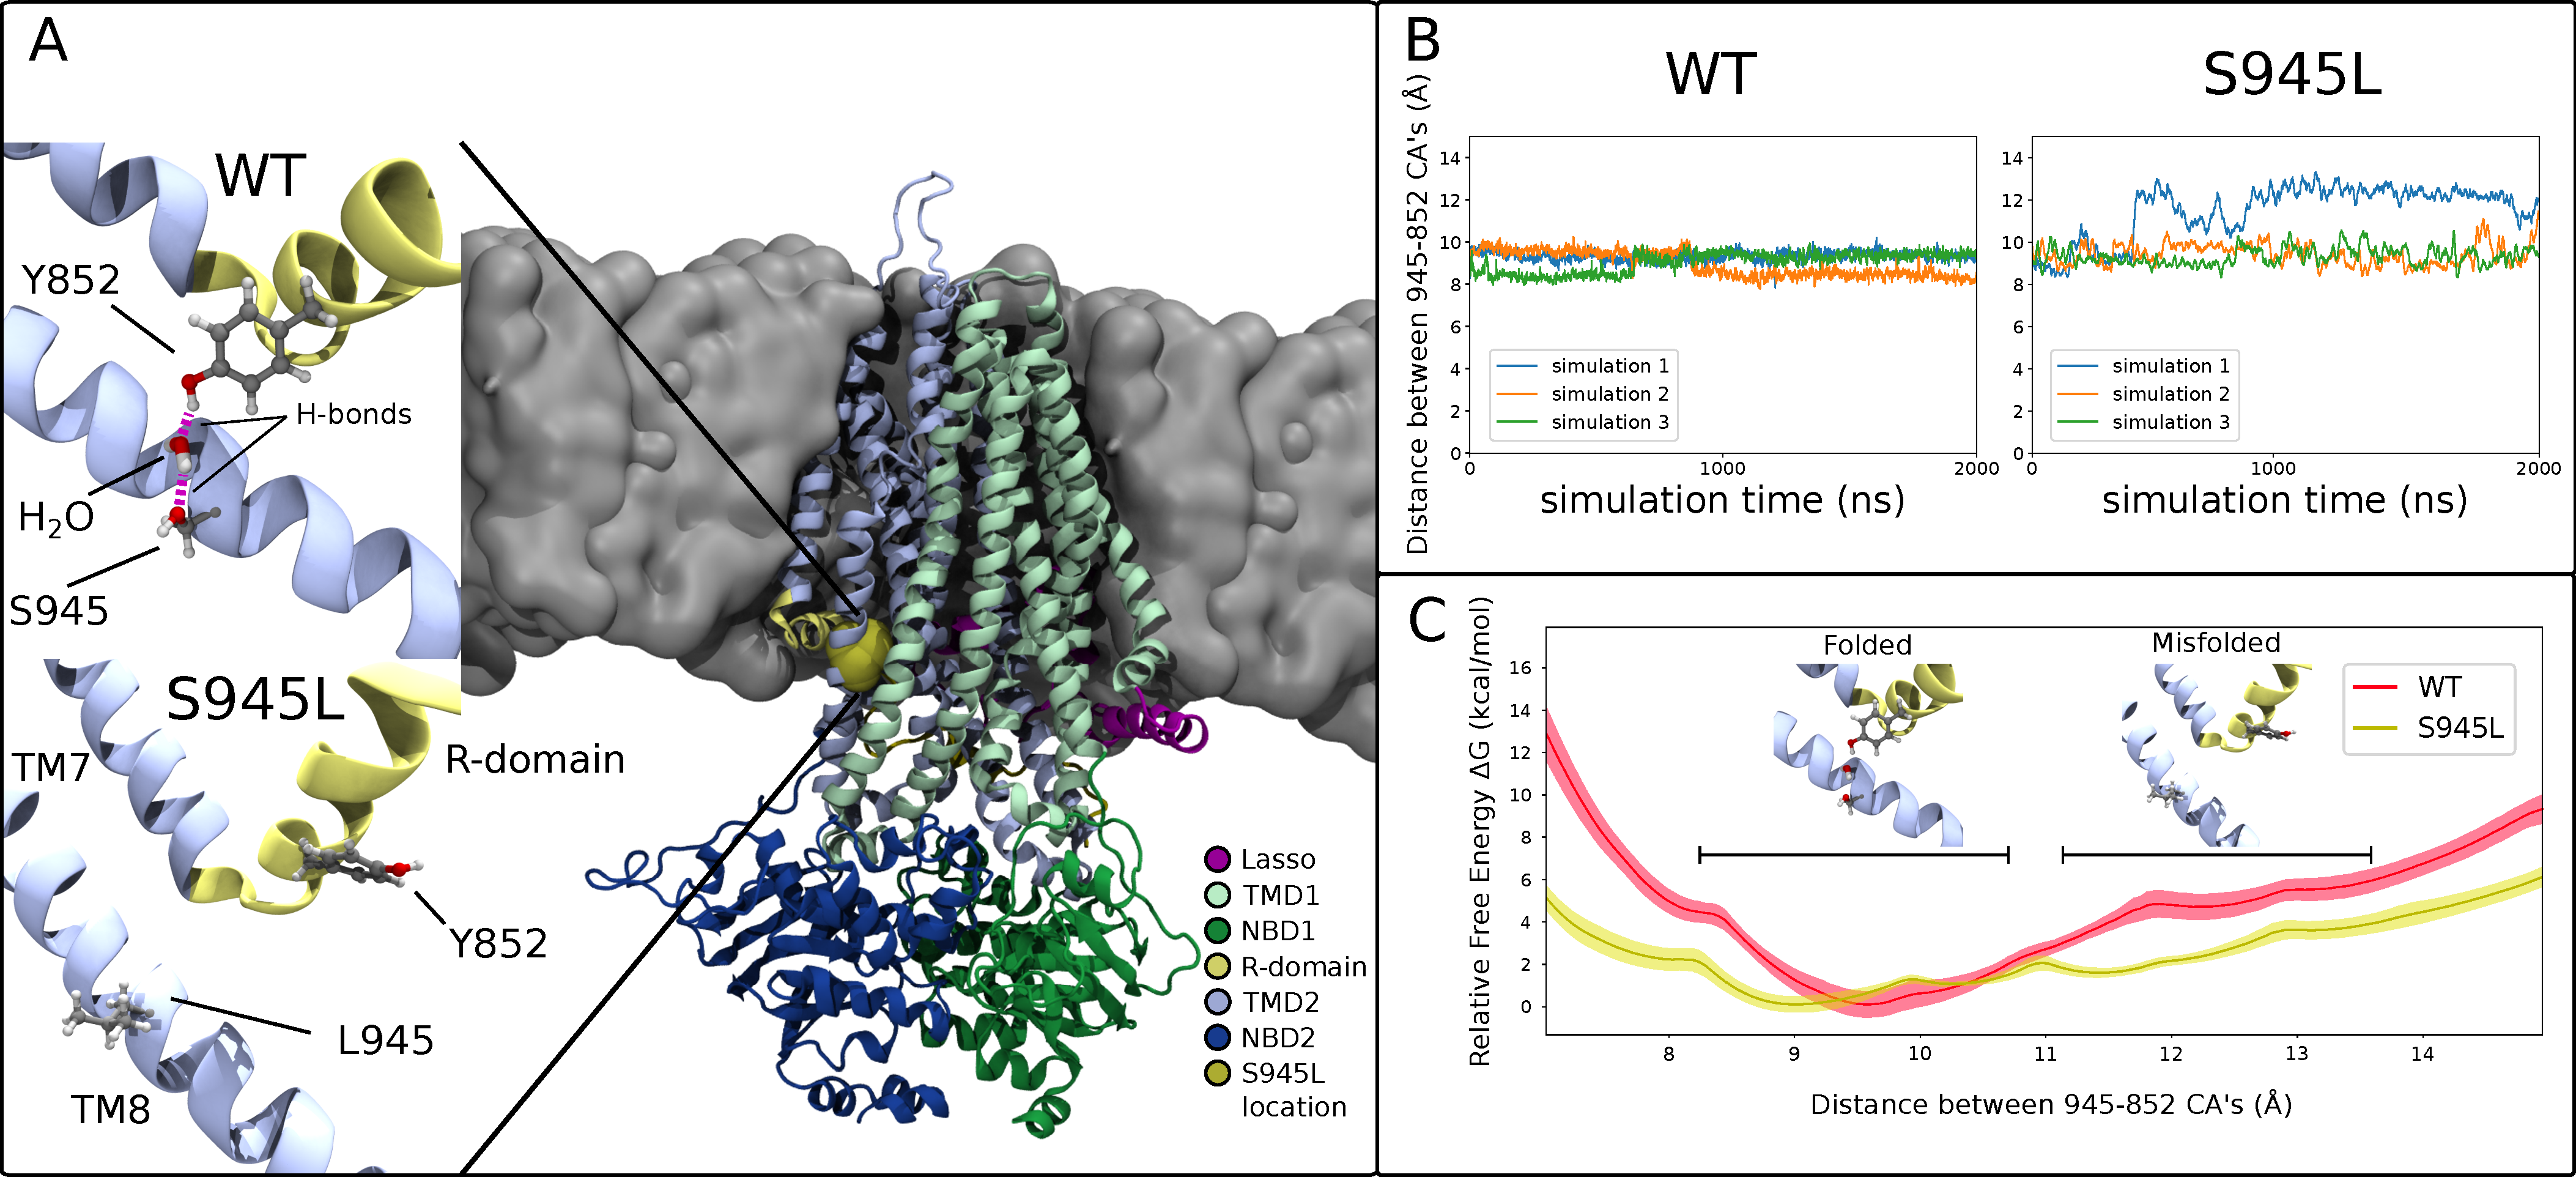
\includegraphics[width=\textwidth]{figures/S945L/Figure1_MD_03082022.pdf}
\end{center}
	\captionsetup{singlelinecheck = false, justification=raggedright}
\begingroup
\captionof{figure}[S945L] {\textbf{S945L}}{A) The location of the S945L mutation in the open structure of CFTR (PDB ID: 6MSM) is indicated with yellow spheres. It is placed between TM8 and the R-domain, the latter domain is critical for the gating of the channel. B) Data from unbiased simulations of WT and S945L-CFTR. A stable network of hydrogen bonds forms spontaneously in simulations 1, 2 and 3 of WT-CFTR. This interaction connects Y852 to S945. In the S945L mutation, the leucine side chain cannot support this hydrogen-bond network. In simulation 1 of S945L-CFTR, after a conformational transition, the amino acids remained at an average distance of 12.2$\pm$0.7 $\angs$. This is significantly further than the average distance in the WT data: 9.1$\pm$0.3 $\angs$. No significant changes were observed in simulations 2 and 3 of S945L-CFTR. C) Results from umbrella sampling, a more computationally rigorous approach, confirm the presence of the conformational change in S945L-CFTR. Distances below roughly 10.5 $\angs$ correspond to a well folded state, while distances larger than 11 $\angs$ appear to correspond to a poorly folded state. In the mutant, there is a shallow free energy minimum at 11.4 $\angs$ with a difference in the energy landscape of 3.2 kcal/mol compared to WT-CFTR at the same location. The presence of this shallow free energy minimum indicates that S945L-CFTR is more likely to misfold than WT-CFTR. }
\label{S945L_MD_1}
\endgroup

\section{Discussion}
We have described in detail the structural and functional CFTR defects caused by the S945L mutation. In silico protein modelling via MD simulations was used to determine the molecular cause of both a folding and a gating defect in S945L-CFTR.  Airway epithelial cell models derived from a participant with S945L/G542X-CFTR were also created and their response to CFTR modulators was tested via functional studies, to characterise their functional defect. The rescue of mutant CFTR was found to then translate to success in the clinic, as the patient carrying this mutation had an increase in lung function following the administration of the recommended therapy.

In our MD simulations of WT-CFTR, a stable network of hydrogen bonds linking Y852 in the R-domain to S945 on TM8 was identified. This interaction was not visible in the cryo-EM structure of the channel, where S945 faced away from Y8528. It is often not possible to resolve such water mediated interactions in cryo-EM structures. This is due to the difficulties in achieving a high enough resolution with experimental structural biology techniques and the dynamic nature of the proteins themselves. The elucidation of this interaction in this study demonstrates the atomistic insight which computational methods can provide into the function of proteins. In simulations of S945L-CFTR, this interaction was disrupted, and our results indicate that the R-domain may move away from TM8 (Figure \ref{S945L_MD_1}B). Due to the importance of the R-domain in gating, we expect that a change to its position will give rise to a gating defect. This is a similar mode of pathogenesis the one observed in the I37R mutation, although it is interesting that it occurs in a different domain in CFTR. Simultaneously, the disruption of this link between two different domains is likely to give rise to a folding defect, as the elbow region will be less likely to fold correctly. Hence, our MD simulations have revealed a unique mode of pathogenesis for the S945L mutation. It is unlikely that other mutations would disrupt this hydrogen bond in the same way. This is another example in a set of MD simulations of the CFTR protein which suggest that CFTR modulators can elicit a response in many missense mutations, each with unique molecular phenotypes \cite{wong2022,wong2022a,billet2020,sabusap2021}. 

The results from clinical and \textit{in vitro} experiments are not shown explicitly, but described here to complement and give context to our MD studies. When tested under basal conditions, the S945L/G542X-CFTR ALI cell models exhibited high residual activity. This indicated the presence of some CFTR protein at the cell surface, suggesting that the S945L mutation produces a mild CFTR folding defect. Monotherapies using either a single potentiator or a single corrector were not able to restore CFTR function to levels which would indicate clinical benefit. However, combination therapies Symdeko and Trikafta were able to restore function in these cell models. This was expected as Trikafta has recently been evaluated in rare class II CFTR folding mutations and variable genotype-specific responses were found \cite{veit2020, laselva2021}. Like the prototypical class II folding mutation $\Delta$F508, S945L has been reported to cause multiple defects including protein maturation, channel gating and conductance \cite{seibert1996}. 

We correlated the \textit{in vitro} drug response of the S945L/G542X-CFTR patient-derived cell models to the patient’s in vivo change in lung function (FEV1) following treatment with the Symdeko. Once the patient was administered Symdeko for 12 months, their lung function improved. These results support the use of personalised primary airway cell models as a valuable tool to study modulator efficacy and predict patient drug response for patients who carry rare mutations which are difficult to study through clinical trials. 

The \textit{in vitro} and clinical studies demonstrate the efficacy of pre-clinical cellular models, while the MD studies demonstrate the rescue of yet another unique molecular defect by CFTR modulators.  

\textit{In vitro}, S945L-CFTR was not found to respond to treatment by a potentiator monotherapy. This is consistent with previous findings. The rescue of S945L-CFTR by correctors has not previously been assessed, but again significant restoration was not observed with this kind of monotherapy. By contrast, combination therapies Trikafta and Symdeko were found to restore function in cellular models. As such, we characterise S945L to incur both CFTR folding and gating defects, which is in support of previous molecular studies performed in heterologous expression CHO cells \cite{seibert1996}, as well as the findings of our MD simulations.

Since the response of different CFTR mutations \cite{laselva2021} to modulators is heterogeneous \cite{wainwright2015,boyle2014}, there is a strong rationale for modulator screening of CFTR in patient-specific cell models. Prediction of CFTR drug response in patient-specific cell models may, in the future, lead to extended approval of CFTR modulators for rare CFTR mutations currently without treatment access. Together with other integrative studies using both MD simulations and \textit{in vitro} functional studies to characterise CFTR mutations and predict drug response in a personalised manner \cite{wong2022,wong2022a,billet2020,sabusap2021, sharma2015}, there is a growing body of evidence that a large number of unique molecular defects may be rescued by CFTR modulators. Further development of patient-specific cell models as a predictive tool could lead to the optimal choice of CFTR modulators to treat each patient.  

\section {Supplementary Information}
\renewcommand{\thefigure}{\arabic{chapter}.S\arabic{figure}}
\setcounter{figure}{0}

\begin{center}
	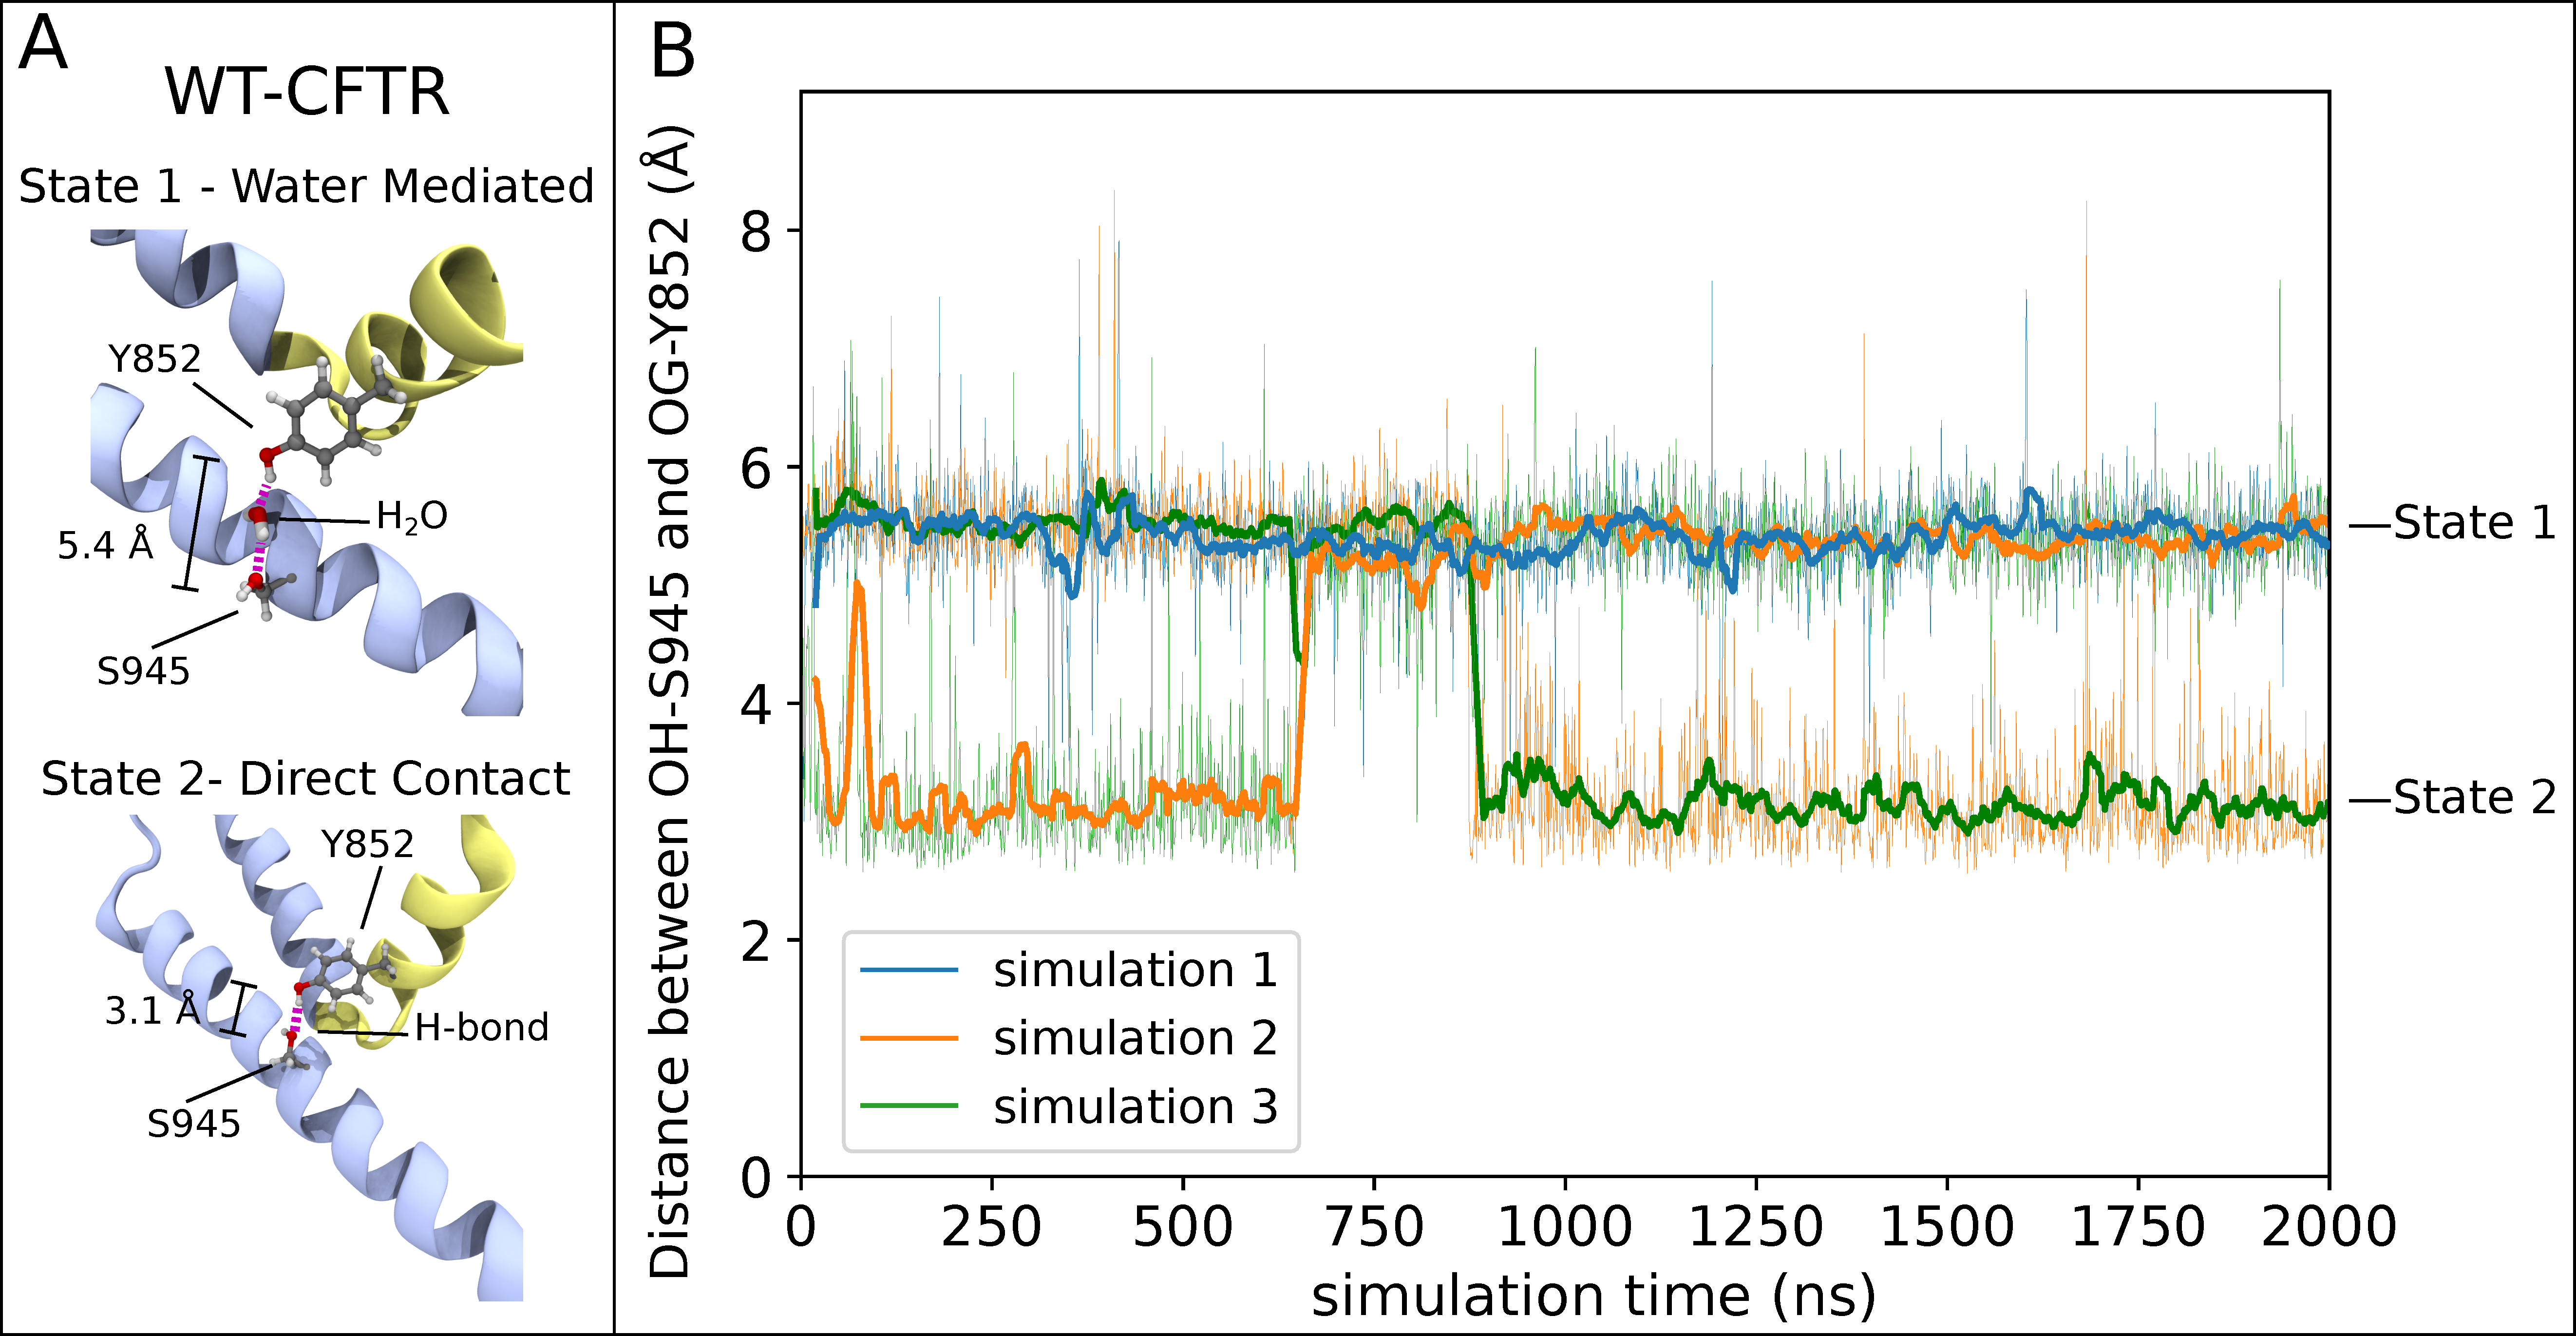
\includegraphics[width=\textwidth]{figures/S945L/supp1_MD.pdf}
\end{center}
	\captionsetup{singlelinecheck = false, justification=raggedright}
\begingroup
\captionof{figure}[Detailed View of the Hydrogen Bond Netowrk in WT-CFTR] {\textbf{Detailed View of the Hydrogen Bond Netowrk in WT-CFTR}}{A. In our simulations we observe two possible states. State 1 occurs when a water molecule stably mediates the interaction between the sidechains of S945 and Y952. State 2 occurs when they are in direct contact with each other. B. The distance between the oxygen atoms in the polar side chains of S945 and Y852 throughout the WT simulations. In simulation 1 the system remains in state 1 throughout. Simulation 2 begins in state 1 but transitions to state 2 at 900 ns. Simulation 3 begins in state 2 but transitions to state 1 at 700 ns. Data is graphed with a 20 ns moving average to more clearly delineate the difference between the two states. This data indicates that the two states each contribute to the stable hydrogen bond network between Y852 and S945.}
\label{S945L_MD_S1}
\endgroup

\begin{center}
	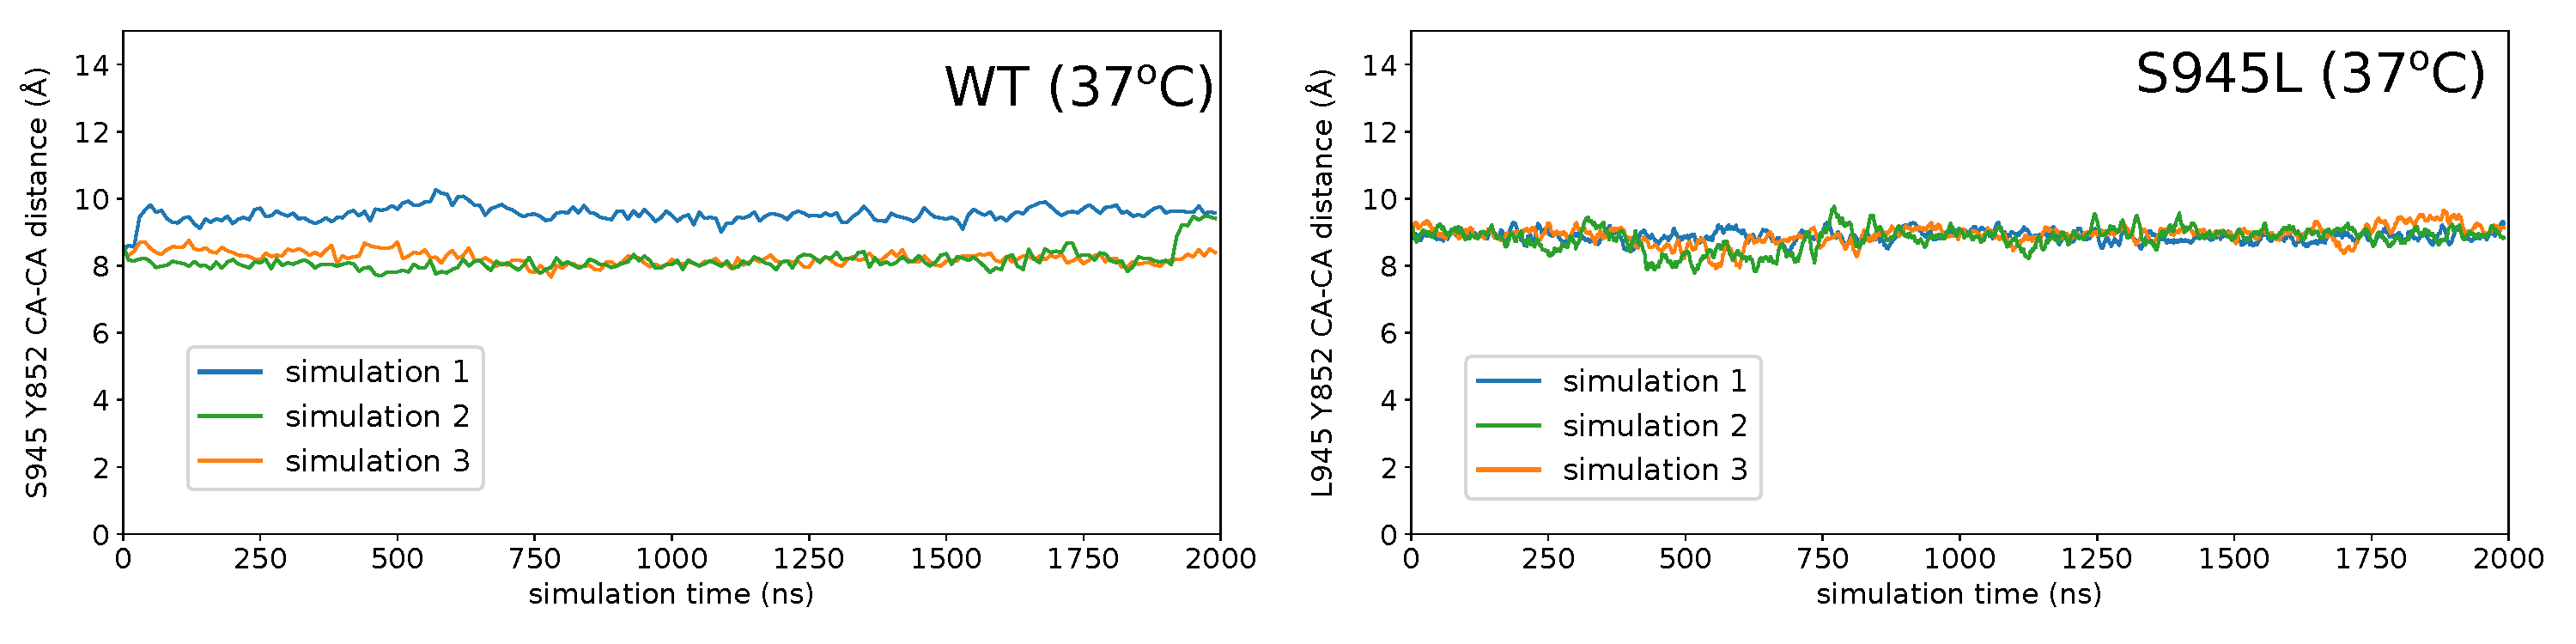
\includegraphics[width=\textwidth]{figures/S945L/310K_supp.pdf}
\end{center}
\captionsetup{singlelinecheck = false, justification=raggedright}
\begingroup
\captionof{figure}[Simulations of WT-CFTR and S945L-CFTR at Physiological Temperature] {\textbf{Simulations of Both WT-CFTR and S945L-CFTR at Physiological Temperature ($37^o$C)}}{In the WT data, we again see a stable interaction between Y852 and S945. The simulations 2 and 3 remain in state 2 throughout the whole simulation, with simulation 2 changing to state 1 at roughly 1900 ns. Simulation 1 quickly transitions to state 1 and remains there throughout the simulation. In S945L, the presence of the lipid bilayer has slowed down the kind of conformational changes we would expect from a mutation like S945L. Unfortunately, no pathogenic motions were visible at physiological temperatures on the timescales accessible with unbiased MD simulations. The Y852 and L945 amino acids remained at a distance somewhere between state 1 and state 2. These results motivated a more rigorous study with umbrella sampling in order to understand the molecular details of the defect which the S945L mutation causes to CFTR. }
\label{S945L_MD_S2}
\endgroup

\begin{center}
	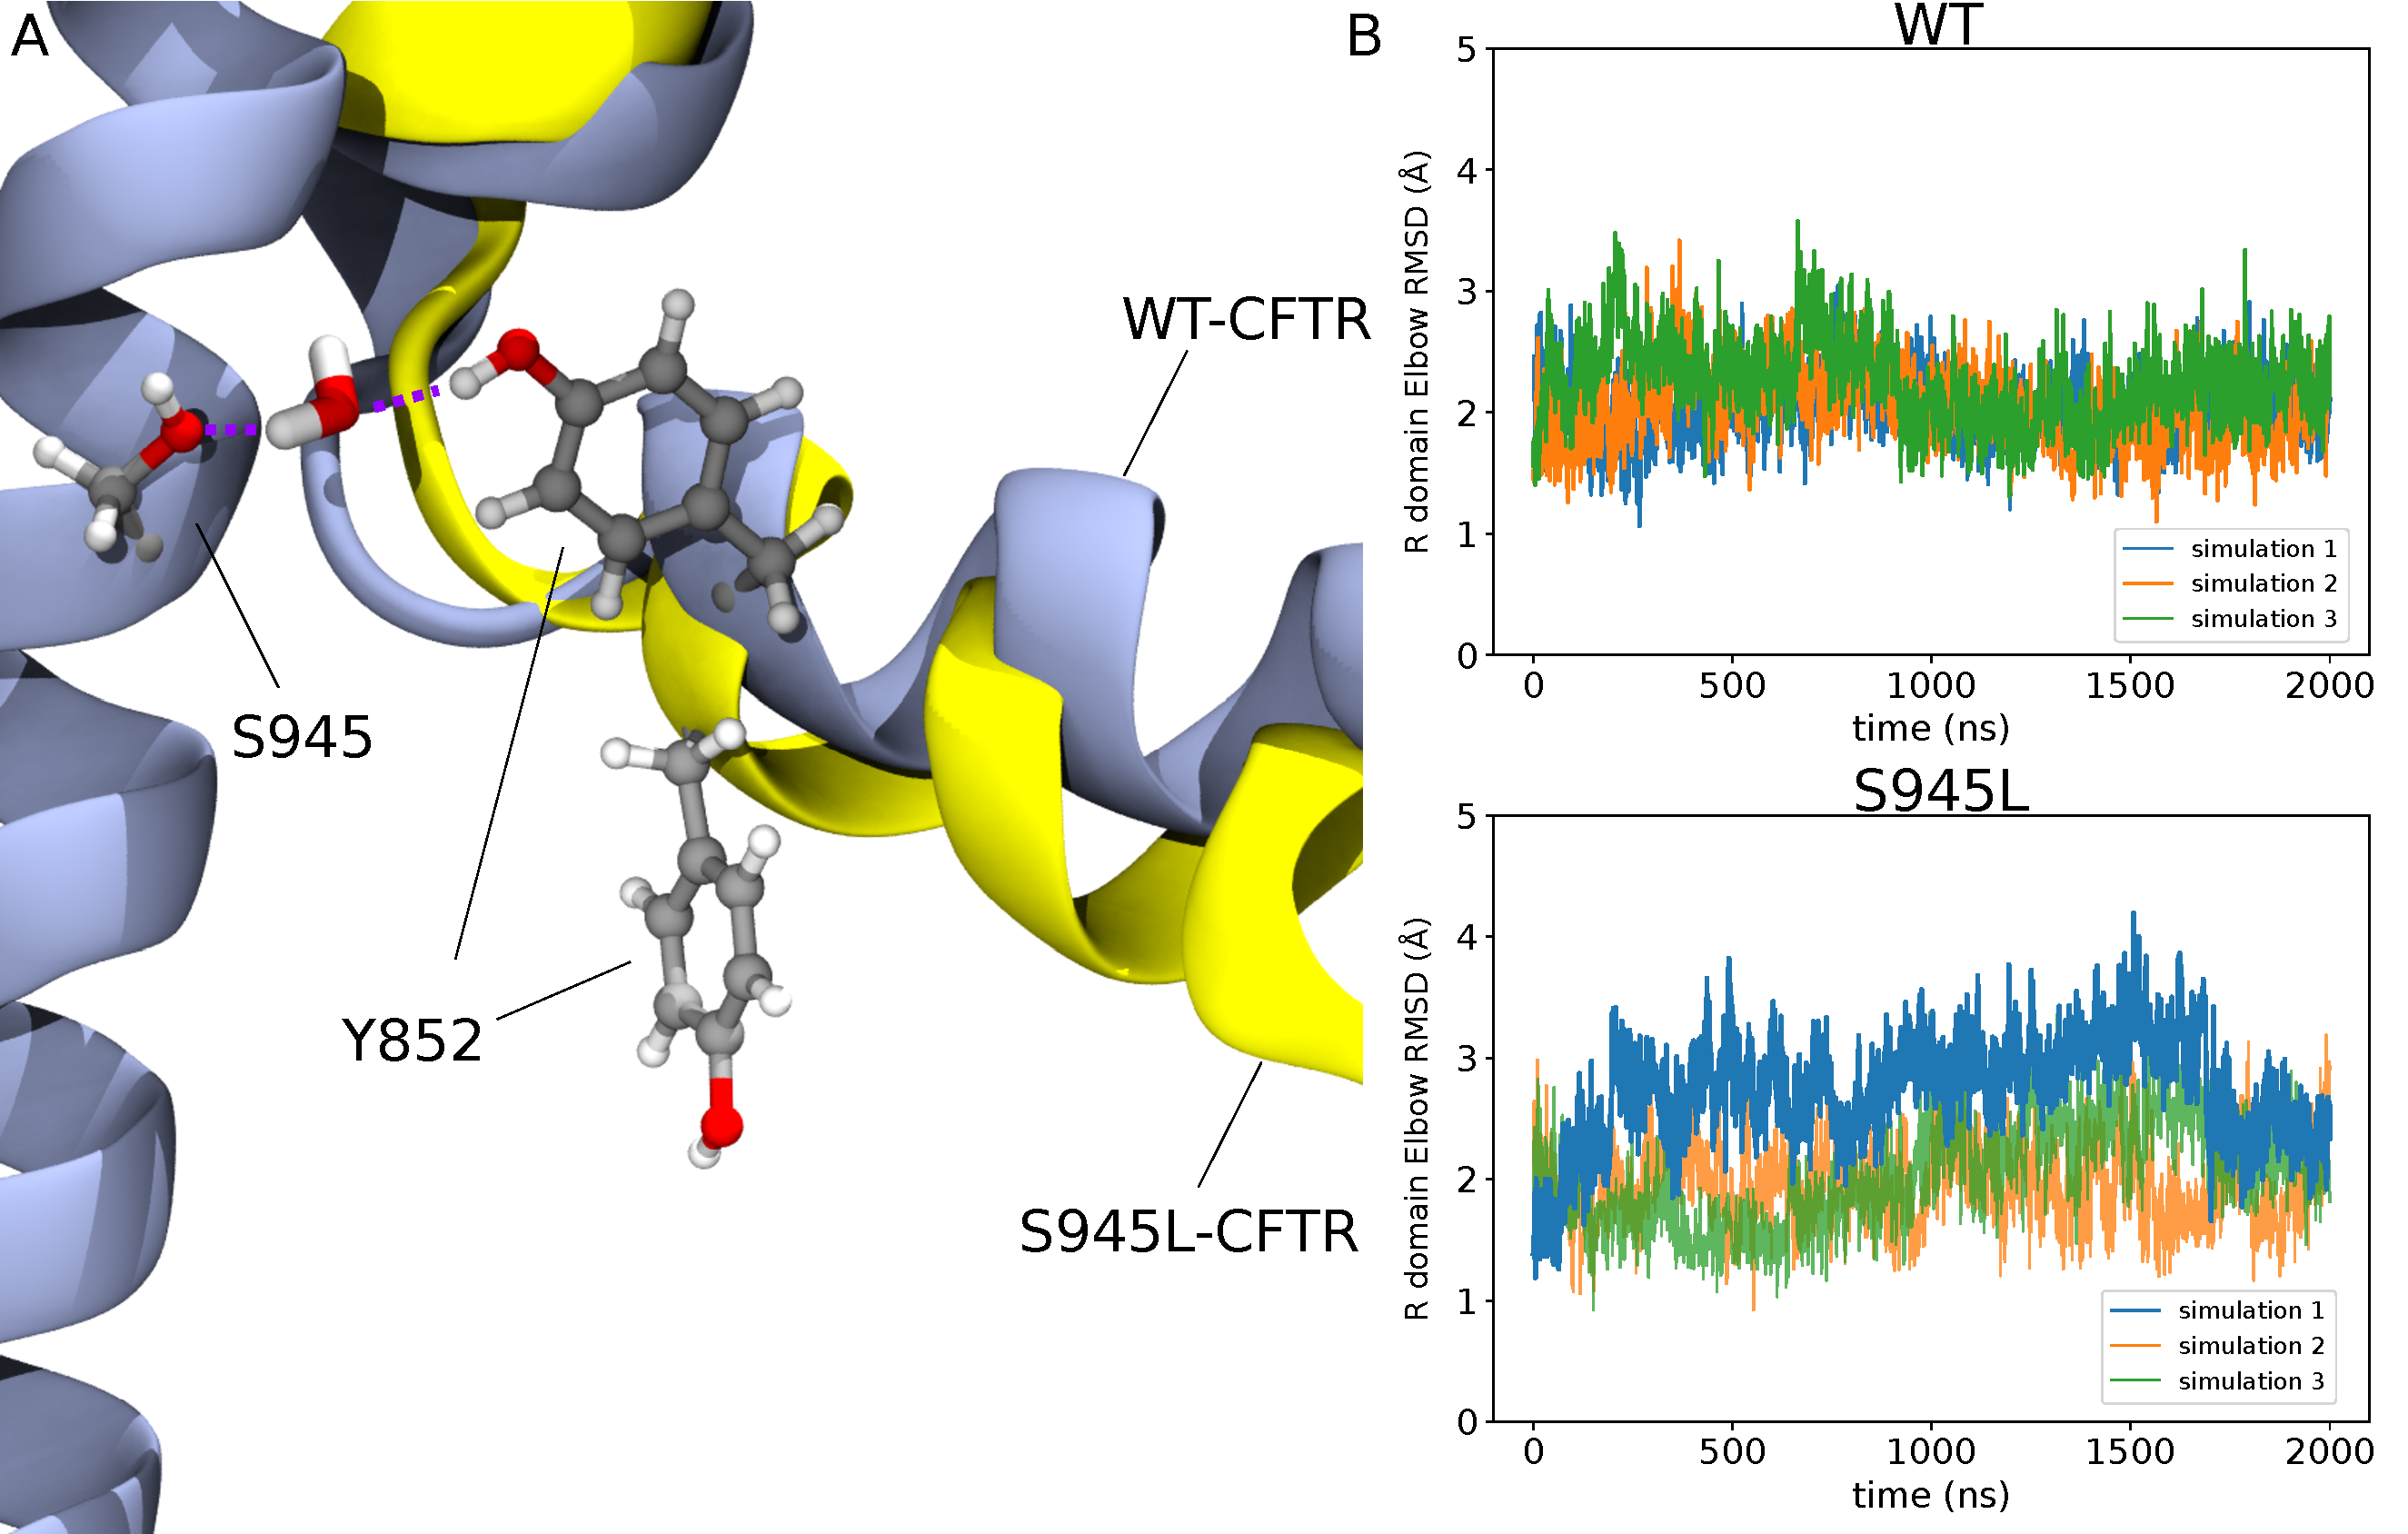
\includegraphics[width=\textwidth]{figures/S945L/supp3_MD.pdf}
\end{center}
\begingroup
\captionsetup{singlelinecheck = false, justification=raggedright}
\captionof{figure}[Local Conformational Change of the Elbow Between TM8 and the R-domain. ] {\textbf{The Local Conformational Change of the Elbow Between TM8 and the R-domain.}}{(WT-purple, S945L-yellow) A. The Y852 side chain sits in the elbow of the R-domain (amino acids 845-886) and when it is perturbed, a shift in the elbow is observed. This conformational change is proposed to influence the gating cycle of CFTR. B. The Root Mean Squared Deviation (RMSD) values of the elbow region, calculated with reference to the alpha Carbon Atoms of the 6MSM structure. Simulation 1 was the replicate with the greatest perturbation compared to the WT structure in the unbiased simulations (Figure \ref{S945L_MD_1}B). The data for simulation 1 of the S945L mutation indicates a destabilisation of this elbow region. This is proposed to cause defects with both the gating cycle of the protein and the stability of the correctly folded state.}

\label{S945L_MD_S3}
\endgroup


\section{Method Details}
\subsection{Molecular Dynamics}
2.1 Molecular Dynamics
The CFTR protein model used for molecular dynamics simulations was based on the ATP-bound human CFTR cryogenic electron microscopy (cryo-EM) structure (PDB ID: 6MSM) \cite{zhang2018}. The construction of the CFTR protein system, including the modelled part of the R domain, has been described previously \cite{wong2022}. In brief, the CFTR model was embedded in a simplified cell membrane model containing pure 1-palmitoyl-2-oleoyl-sn-glycero-3-phosphocholine (POPC) lipids then solvated with 150 mM KCl on both the cytoplasmic and periplasmic sides.

In this study, the software Gromacs v2021.1 \cite{abraham2015} was used for all MD simulations. Molecular mechanics parameters were supplied via the CHARMM36m \cite{huang2016} force field with the following modifications for faster simulation performance: virtual site topologies \cite{feenstra1999} for all molecules while using MkVsite36 to generate topologies for the ATP molecules \cite{larsson2020}, as well as parameter adjustments specific to lipids \cite{olesen2018}. The initial positions of all molecules were equilibrated for production runs in two phases: first via energy minimisation using a steepest descent algorithm, then followed by a 6 ns simulation where position restraints were imposed on all non-hydrogen atoms and then gradually relaxed. 

A series of 2 $\mu$s Production MD simulations were carried out with three replicates for each of WT and S945L-CFTR. To decrease computational expense, elevated temperatures of 350 K were used (77°C) to accelerate conformational transitions. The use of elevated temperatures to study defects in mutant CFTR was validated previously \cite{wong2022}. All measurements of Root Mean Squared Deviation (RMSD) were calculated using the positions of alpha carbons in the 6MSM PDB structure 8 as a reference. 

\subsection{Umbrella Sampling Protocols}
The free energy surfaces were constructed by measuring the potential of mean force (PMF) profile between the amino acids Y852 and S/L945. The distance between the alpha carbon atoms in these amino acids was used as the collective variable for the calculation. This distance was varied from 6-16 $\mbox{\angs}$ with a restraint of 10 kcal/mol/$\mbox{\angs}^2$. Umbrella sampling simulations were performed in 10 windows spaced 1 $\mbox{\angs}$ apart. After 100 ns of equilibration for each window, 100 ns of data were collected. The resultant PMF profiles were calculated from the average of the 5 profiles determined from 5 independent samples of 20 ns each. Uncertainties for this result were calculated as twice the standard error of the mean for these 5 samples. The calculations have clearly converged, demonstrated by uncertainties of less than 1 kcal/mol in the free energy surfaces of both the WT and S945L-CFTR. Plumed 2.6 \cite{bonomi2009, tribello2014, bonomi2019} was used to perform the umbrella sampling, and WHAM \cite{grossfield2012} was used to calculate the PMF profiles. 
